\documentclass[thmsb,11pt]{article}
\usepackage{amsfonts}
\usepackage{appendix}
\usepackage[pagewise,displaymath, mathlines]{lineno}
\usepackage{amssymb}
\usepackage{amsmath}
\usepackage{graphicx}
\usepackage{color}
\usepackage{refcount}
\usepackage{natbib}
\usepackage{bm}
\usepackage{hyperref}
\usepackage{epstopdf}
\setcounter{MaxMatrixCols}{10}
\newtheorem{theorem}{Theorem}
\newtheorem{acknowledgement}[theorem]{Acknowledgement}
\newtheorem{algorithm}[theorem]{Algorithm}
\newtheorem{assumption}{Assumption}
\newtheorem{axiom}{Axiom}
\newtheorem{case}[theorem]{Case}
\newtheorem{claim}[theorem]{Claim}
\newtheorem{conclusion}[theorem]{Conclusion}
\newtheorem{condition}[theorem]{Condition}
\newtheorem{conjecture}{Conjecture}
\newtheorem{corollary}{Corollary}
\newtheorem{criterion}[theorem]{Criterion}
\newtheorem{definition}{Definition}
\newtheorem{lemma}{Lemma}
\newtheorem{problem}[theorem]{Problem}
\newtheorem{proposition}{Proposition}
\newtheorem{solution}[theorem]{Solution}
\newtheorem{summary}[theorem]{Summary}
\newtheorem{example}{Example}
\newtheorem{exercise}{Exercise}
\newtheorem{notation}{Notation}
\newtheorem{remark}{Remark}
\newcommand{\bmat}{\begin{matrix}}
\newcommand{\emat}{\end{matrix}}
\newcommand{\ov}{\overline}
\newcommand{\un}{\underline}
\newcommand{\EE}{\mathbb E}
\newenvironment{proof}[1][Proof]{\noindent \textbf{#1.} }{\  \rule{0.5em}{0.5em}}
\topmargin=-1cm
\oddsidemargin=-0cm
\textheight=22.2cm
\textwidth=16cm
\setcounter{secnumdepth}{2}
\pagestyle{plain}
\setcounter{figure}{0}
%\setpagewiselinenumbers
%\linenumbers
\begin{document}

\title{\textbf{ Redistribution with a continuum of agents}}
\date{}
\maketitle
\section{Introduction}
We study optimal affine taxation in an economy with continuum of agents that face (un-insurable) shocks to their idiosyncratic labor productivities. We first specify the problem without aggregate risk.
\section{Ramsey planner's problem}
Given a joint distribution $\Gamma_0(x_{0},m_{0},e_{0})$ over marginal utilities adjusted assets, scaled marginal  utilities and past productivities, the Ramsey allocation solves the following problem from t$>$0.
\begin{equation}
\label{eq-obj}
\max_{c^i_{t},l^i_t,x^i_t,m^i_t} \sum_{t}\beta^t\int \omega^i  u(c^i_t,l^i_t)di 
\end{equation}

subject to 

\begin{subequations}

\begin{equation}
\label{eq-imp}
\frac{x^i_{t-1}u^i_{c,t}}{\beta\mathbb{E}_{t-1}u^i_{c,t}}=u^i_{c,t}(c^i_t-T_t)+u^i_{l,t}l^i_{t}+x^i_t
\end{equation}


\begin{equation}
\label{eq-Bond_1}
\alpha^1_{t}=m^i_{t}\mathbb{E}_{t}u^i_{c,t+1}
\end{equation}

\begin{equation}
\label{eq-Bond_2}
\alpha^2_{t}=m^i_{t}u^i_{c,t}
\end{equation}

\begin{equation}
\label{eq-wages}
-u^i_{l,t}=(1-\tau_t) u^i_{c,t} e^i_t
\end{equation}


\begin{equation}
\label{eq-productivity}
e^i_t=(1-\nu)\bar{e}+\nu e^i_{t-1}+q\epsilon^i_t
\end{equation}

\begin{equation}
\label{eq-norm-m}
\int m^i_t di=1
\end{equation}



\begin{equation}
\label{eq-resources}
\int l^i_t e^i_t di = \int c^i_t di+g
\end{equation}



\end{subequations}

Equations \eqref{eq-Bond_1} and \eqref{eq-Bond_2} ensure that individual Euler equations hold. The FOCs of this problem are summarized below:
   \begin{subequations}
	   \label{sys-FOC}	   
	   	\begin{equation}
	   	\label{eq-foc_x}
	   	\mu^i_{t-1}=\mathbb{E}_{t-1}\frac{u^i_{c,t}}{\mathbb{E}_{t-1}u^i_{c,t}}\mu^i_t
	   	\end{equation}

	   	 \begin{equation}
	   	 	\label{eq-foc_l}
	   	 	\omega^i u^i_{l,t}-\mu^i_t[u^i_{ll,t}l^i_t +u^i_{l,t}]-\phi^i_t u^i_{ll,t}+\lambda_t e^i_t=0   	
	   	\end{equation}    	


	   	\begin{equation}
	   		\label{eq-foc_m}
	   	   	\rho^i_{2,t}u^i_{c,t}+\rho^i_{1,t}\mathbb{E}_{t}u^i_{c,t+1}+\eta_t=0
	   	\end{equation}


	   	\begin{equation}
	   		\label{eq-foc_c}
	   	  \omega^i u^i_{c,t}+x^i_{t-1}\frac{u^i_{cc,t}}{\beta \mathbb{E}_{t-1}u^i_{c,t}}\left[\mu^i_{t}-\mu^i_{t-1}\right]-\mu^i_t[u^i_{cc,t}c^i_t+u^i_{c,t}]+\beta^{-1}\rho^i_{1,t-1}m^i_{t-1}u^i_{cc,t}+\rho^i_{2,t}m^i_tu^i_{cc,t}-\phi^i_t e^i_t(1-\tau_t)u^i_{cc,t}-\lambda_t=0    	
	   	 \end{equation}


	      \begin{equation}
	      	\label{eq-foc_tau}
	       \int \phi^i_t u^i_{c,t}e^i_t di =0  	
	      \end{equation}       


	   	\begin{equation}
	   	\label{eq-foc_T}
	   	\int u^i_{c,t}\mu^i_tdi=0
	   	\end{equation}  


	        \begin{equation}
	        	\label{eq-for_alpha}
	           	\int \rho^i_{j,t}di=0 \quad j=1,2
	        \end{equation}          



	   \end{subequations}	

The solution to these FOC can be expressed recursively using individual states $\xi^i_{t-1}=[\mu^i_{t-1},m^i_{t-1},e^i_{t-1}]$, shocks $\epsilon^i_t$ and aggregate state $\Gamma_{t-1}(\xi^i_{t-1})$. 

\section{Ricardian Equivalence}
Note that, using equation \eqref{eq-Bond_1}, equation \eqref{eq-foc_T} can be rewritten as 
\[
	\int \frac{\mu^i_t}{m^i_t} = 0
\]  Moreover, equation \eqref{eq-foc_x} can be expressed as
\[
\frac{\alpha^1_{t-1} \mu^i_{t-1}}{m^i_{t-1}} = \alpha^2_t \EE_{t-1} \frac{\mu^i_t}{m^i_t}
\]By integrating both sides with respect to $i$, we obtain
\[
	\alpha^1_{t-1} \int \frac{\mu^i_{t-1}}{m^i_{t-1}}di = \alpha^2_t\int \frac{\mu^i_{t}}{m^i_t} di
\]  This implies that if 
\[
	\int \frac{\mu^i_{t-1}}{m^i_{t-1}} = 0
\]is satisfied for time $t-1$ we have then
\[
	\int \frac{\mu^i_t}{m^i_t} = 0
\] thus equation \eqref{eq-foc_T} is redundant and we can choose $T$ to be any value.  For simplicity we set $T=0$.

\section{Optimal Taxes}
In this section we derive a simple expression for taxes and use it to examine how the Ramsey plan uses distortionary taxes to redistribute inview of inequality in earnings and wealth.  

The FOC for labor \eqref{eq-foc_l} can be re-written as 


 \[
\omega^i u^i_{c,t}\frac{u^i_{l,t} e^i_t}{u^i_{ll,t}}- \mu^i_t u^i_{c,t}e^i_t[l^i_t +\frac{u^i_{l,t}}{u^i_{ll,t}}]+\frac{\lambda_t u^i_{c,t}(e^i_t)^2}{u^i_{ll,t}}=\phi^i_tu^i_{c,t}e^i_t    	
\]

 Suppose $u(c,l)=\frac{c^{1-\sigma}}{1-\sigma}-\frac{l^{1+\gamma}}{1+\gamma}$. The above expression simplifies to


 \[
\frac{ \omega^i u^i_{c,t}y^i_t}{\gamma}- \mu^i_t u^i_{c,t}y^i_t[1 +\frac{1}{\gamma}]-\lambda_t\gamma^{- 1}\frac{y^i_t }{1-\tau_t}=\phi^i_tu^i_{c,t}e^i_t    	
 \]

Define $w_{i,t}=u^i_{c,t}[\omega^i-\mu^i_t(1+\gamma)]$ and $\bar{w}_{t} = \int u^i_{c,t}\omega^i di$ and $\bar{w}_{i,t}=\frac{w_{i,t}}{\bar{w}_t}$.

Integrating  over i's we have

 
\begin{equation}
	\label{eq-labor_taxes}
\frac{1}{1-\tau_t}=\frac{\hat{Y}_t}{Y_t} \frac{\bar{w}_t }{\lambda_t}
\end{equation}   

Where $Y_t=\int y^i_t di$ and $\hat{Y}_t=\int y^i_t \bar{w}_{i,t}di$
\subsection{Special cases}
With quasilinear utility and absent non-negativity constraints, we have a simple expression for how taxes depend on the distribution of initial Pareto weights.

 
\begin{equation}
	\label{eq-ql-taxes}
\frac{1}{1-\tau}=\frac{\hat{Y}}{Y}	
\end{equation}   

where $\bar{w}^{i}_t$ weights used in computing $\hat{Y}$ are given by $1+\gamma(\omega^i-1)$. We can quickly draw some implications from this. 
\begin{itemize}
\item Taxes are constant through time.
\item If $\omega^i=1$, taxes are zero.
\item Suppose productivities are iid over time,  taxes will be close to zero.
\item Suppose productivities have a permenant component, taxes will be positive if agents with high productivities have low pareto weights and vice versa
\end{itemize}
\subsection{Risk aversion}


With risk aversion we have spreads in marginal utilities. This generates a desire to use transfers even if $\omega^i=1$.To examine this in detail conisder two extreme economies. The first has iid productivity shocks $(\rho=0)$ and the second one has permenant productivity shocks $(\rho=1)$\footnote{XXX stationarity}.


The term  $\frac{\bar{w}_t }{\lambda_t}$ captures increase in the welfare from transfers relative to the value of resources (note $\lambda$ is a multiplier on the resource constraint.) Thus a higher value for this term would imply larger role of taxes and the consequent transfers. 

The first term $\frac{\hat{Y_t}}{Y_t}$ is increasing in the covariance between $\bar{w}^i_t$ and pre-tax  labor earnings $y^i_t$. Notice that these weights $\bar{w}^i_t$ are decreasing in the multiplier on the budget constraint of agent $i$ : $\mu_t^i$. 

Consider the case where shocks to productivities are predominatly transitory.   Agents save most of the shock for precautionary reasons. Overtime the agents with a unlucky stream of shocks will have lower wealth and low consumption and lower leisure. This will imply a lower $\bar{w}^i_t$ and higher $y^i_t$ for such agents. The optimal response of government is to lower taxes and possibly give labor tax subsidies. 

In the case where productivities have a permenant component, the output $y^i$ will be higher for productive agents. These agents will also have higher wealth shares. This would make $y^i_t$ and $\bar{w}^i_t$ positively correlated and call for higher taxes. 

The next two sections describe the  algorithm for computing an approximation for the Ramsey allocation for this economy.

\section{Deterministic Steady State}
We first look at an economy with $q=0$. Given a joint distribution $\Gamma_0(\xi)$ the non-stochastic steady state is described by an allocation $c(\xi), l(\xi), x(\xi)$ and aggregate labor taxes $\tau$. 

Suppose $\Gamma_0(\xi)$ satisfies the following two properties
   \begin{subequations}
   \label{sys-gamma_0_prop}
	\begin{equation}
	\int m^i di=1
	\end{equation}
	\begin{equation}
	\int \frac{\mu^i}{m^i} di=0
	\end{equation}
   \end{subequations}
Given this we can conclude that the FOC can be satisfied with $\alpha^1=\alpha^2$, $\eta=0$ and $\rho^i_{1}=-\rho^i_2$. To obtain the deterministic steady state we add a few auxiliary variables $\phi(\xi)$,$\rho_1(\xi)$ and aggregates $\lambda$ and $\alpha$. The steady state is given by the following set of equations.  The first set solves for individual policies for a guess of $(\alpha,\lambda,\tau)$ and the second set solves the aggregates

   \begin{subequations}
   \label{sys-steady-state-deterministic-individial}
   	\begin{equation}
   	\label{eq-ss_1}
   	\alpha=m^i u^i_c
   	\end{equation}

	\begin{equation}
   	\label{eq-ss_2}
   	-u^i_l=(1-\tau)u^i_ce^i
   	\end{equation}
   	
\begin{equation}
   	\label{eq-ss_3}
   	\gamma \phi^i = l^i[\omega^i -\mu^i(1+\gamma)] +\frac{\lambda e^i}{u^i_{ll}}
   	\end{equation}

   	
\begin{equation}
   	\label{eq-ss_4}
	   	   u^i_{c}[\omega^i-\mu^i(1-\sigma)]+\rho^i_{1}m^i u^i_{cc}(\beta^{-1}-1)-\phi^i_t e^i(1-\tau)u^i_{cc}-\lambda=0    	
   	\end{equation}
   \end{subequations}
The aggregates $(\alpha,\tau,\lambda)$ solve
   \begin{subequations}
   \label{sys-steady-state-deterministic-aggregates}
   	\begin{equation}
   	\label{eq-ss_agg_1}
   	\int l^i_t e^i_t di = \int c^i_t di+g
   	\end{equation}
	
	\begin{equation}
   	\label{eq-ss_agg_2}
	\frac{1}{1-\tau_t}=\frac{\hat{Y}_t}{Y_t} \frac{\bar{w}_t }{\lambda_t}   	
   	\end{equation}

	\begin{equation}
   	\label{eq-ss_agg_3}
   	\int \rho^i_1 di=0
   	\end{equation}

   \end{subequations}

  \section{Approximation}
%   
% {\color{blue}
%   Collect the individual policy rules in $y(\epsilon|\xi,\Gamma,q)$ and the aggregates as $Y(\Gamma)$. The laws of motion for the state variables are defined by $\xi'(\epsilon|\xi,\Gamma,q)$ and $\Gamma'=\Gamma(\Gamma,q)$.
% \begin{enumerate}
% 
% 
% \item What is the goal ?
% 
%   The goal is to obtain an approximation of the individual policy rules and aggregate variables using pertubation around $q=0$ for an aribrary choice of $\Gamma$. Thus even with a first order exapansion, how agents respond to shocks will depend both on the aggregate distribution  $\Gamma$ and individual state variables $\xi$
% 
% \item What are the challanges
% 
%   \begin{itemize}
%   \item Agggregating across agents 
%   \item Forecasting future aggregate variables
%   \item Accounting for GE effects of higher order terms
%   \end{itemize}
% 
% \item What are the ``tricks'' ?
%   \begin{itemize}
%   \item Exploiting that the steady state is a complete market economy where individual state variables are stationary
%   \end{itemize}
% 
% 
% 
% \item How is it actually implemented ?
% 
% \item Remarks - what are the class of problems this can work? extensions etc
% 
% \end{enumerate}}


For the individual variables let $y$ be the control variables, $\xi$ be the  state variables, and  $\epsilon$ be the idiosyncratic shock.  The aggregate state of the economy is described by the distribution $\Gamma$ over $\xi$, and $Y$ is defined to be the aggregate control variable.  The system of equations that defines our model can be separated into two parts
\begin{equation}\label{eq.ind_con}
	F(y_t, \EE_{t-1} y_t, Y_t, \EE_t y_{t+1} ,\epsilon_t| \xi_{t-1},q,\Gamma_t) = 0  \text{  for all $\xi_{t-1}$}
\end{equation}and
\begin{equation}\label{eq.agg_con}
	\int G(y_t,,Y_t,\epsilon_t|\xi_{t-1},q,\Gamma_t) d\Gamma_t(\xi_{t-1})d\epsilon_t = 0
\end{equation}  Here $F$ in equation \eqref{eq.ind_con} represents the constraints on the individual variables while equation \eqref{eq.agg_con} represents the constraints on the aggregate variables.  There are two major differences between this a setup and the standard way of linearizing models.  The first is the aforementioned separation between aggregate and individual constraints.   The second is the inclusion of the term  $\EE_{t-1} y_t$ which allows us to impose the measurability restrictions associated with incomplete markets.  Specifically, $x_{t-1}$ should be independent of the realization of the shock $\epsilon_t$ and $\rho^1_{t-1}$ should be independent of the realization of $\epsilon_{t-1}$.  We want to find the policy functions $y_t= y(\epsilon^i| \xi^i_{t-1},q,\Gamma)$ and  $Y_t = Y(q,\Gamma_t)$ that solve those systems.  As next period's state $\xi_t$ can be written as a subset of the controls $y_t$, the function $y(\epsilon^i| \xi^i_{t-1},q,\Gamma)$ induces a law of motion of the individual 
states $\xi_t = \xi(\xi_{t-1}|q,\Gamma_t)$.  This along with the distribution $\epsilon_t$ allows us to construct the law of motion for the aggregate state $\Gamma_{t+1} = \Gamma(\Gamma_t | q)$.

The key insight to begin this analysis is that at the limit where $q = 0$ the law of motion for the idiosyncratic state variable is identity, that is,
\[
	\xi(\xi_{t-1}|0,\Gamma) = \xi_{t-1}
\] for all $\xi$ and $\Gamma$.  This, in turn, implies that $\Gamma(\Gamma_{t}|0) = \Gamma_{t}$ when $q=0$.  All possible distributions $\Gamma$ are stationary non-stochastic steady states.   We will then use a perturbation approach to approximate locally around a choice of steady state $\Gamma$.

\subsection{Linear Approximation}
We will begin with a linear approximation.  Choose any candidate $\overline \Gamma$ as the steady state around which we will approximate the policy rules.  For convenience we will label each agent by $i\in(0,1)$.  Let $\overline \xi^i$ be the steady state value of $\xi$ for agent $i$.  Similarly let $\hat \xi^i_{t-1}  = \xi^i_{t-1} - \overline\xi^i$ be the deviation from the steady state for agent $i$.  This describes the current aggregate state $\Gamma_t$.  We first want to find the linear approximation $\hat Y_t = Y_t - \overline Y$.  This will be the sum of all the linear contributions of $\hat \xi^i_t$:
\begin{equation}\label{eq.Yhat}
	\hat Y_t = \int dY^i_{\xi} \hat \xi^i_{t-1} di
\end{equation}  Note that here $dY^i_\xi$ depends on the individual steady state value $\overline \xi^i$ as well as the global steady state $\overline \Gamma$.  The linear approximation  $\hat y^i_t = y^i_t -\overline y^i$ is a combination to the linear contributions of $\xi^i_{t-1}$, $\epsilon^i_t$ and the aggregation of the contributions of $\xi^j_{t-1}$ for $j\neq i$, thus
\[
	\hat y^i_t = dy^i_\xi \hat\xi^i_{t-1} +  dy^i_\epsilon q\epsilon^i_t + \int dy^{i,j}_\gamma \hat \xi^j_{t-1} dj
\]  We can simplify this further by realizing that the contribution of $\hat \xi^j_t$ to $\hat \xi^i_t$ come through GE contributions via the aggregate variables.  Thus we can express the linearization of the individual controls as 
\begin{equation}\label{eq.y_hat}
	\hat y^i_t =  dy^i_\xi \hat\xi^i_{t-1} +  dy^i_\epsilon q\epsilon^i_t + dy^i_Y \hat Y_t
\end{equation}  Given that the policy rule for $\hat \xi^i_t$ is stationary at $q=0$ we know that the policy rules for the state variables will be 
\[
	\hat \xi^i_t = \xi^i_{t-1} + d\xi^i_\epsilon q\epsilon^i_t
\]  We can use these to forecast the aggregate variables next period
\[
	\hat Y_{t+1} = \int dY^i_\xi \xi^i_{t} di= \int dY^i_\xi(\hat \xi^i_{t-1}  + d\xi^i_\epsilon q\epsilon^i_t)di = \hat Y_t
\]here use the property that we are integrating over a continuum to integrate out the effects of $\epsilon^i_t$ which are mean zero.  Thus, the forecast of future controls satisfies
\[
	\EE_t \hat y^i_{t+1} = dy^i_\xi \hat\xi^i_{t-1}  + dy^i_Y \hat Y_t + dy^i_\xi d\xi^i_\epsilon q\epsilon^i_t	
\]Differentiating the constrain in equation \eqref{eq.ind_con} an constructing the projection matrix $I^\xi_y$ such that $\hat xi^i_t = I^\xi_y \hat y^i_t$ we obtain
\[
	F^i_y\hat y^i_t + F^i_{Ey}\EE_{t-1}\hat y^i_{t} + F^i_Y \hat Y_t + F^i_{Ey'} \EE_t\hat y^i_{t+1} + F^i_\epsilon q\epsilon^i_t + F^i_\xi \hat \xi^i_{t-1} = 0
\]We can then plug in the formulas described above and combine like terms to derive the expressions
\begin{subequations}
\begin{equation}
	dy^i_\xi = -(F^i_y + F^i_{Ey} + F^i_{Ey'})^{-1}F^i_\xi \hat\xi^i_{t-1}
\end{equation}
\begin{equation}
	dy^i_\epsilon = -(F^i_y + F^i_{Ey'} dy^i_\xi I^\xi_y)^{-1} F^i_\epsilon 
\end{equation}
\begin{equation}
	dy^i_Y = -(F^i_y + F^i_{Ey} + F^i_{Ey'})^{-1} F^i_Y
\end{equation}
\end{subequations}Finally, we can use the aggregate constraints
\[
	\int\left[ G^i_y \hat y^i_t + G^i_Y \hat Y_t+ G^i_\xi \hat \xi^i_{t-1}\right]di = 0
\]to obtain
\begin{equation}
	dY^i_\xi =- \left(\int G^i_y dy^i_Y + G^i_Ydi\right)^{-1}\left(G^i_y dy^i_\xi + G^i_\xi\right)
\end{equation}
\subsection{A Quadratic Approximation}
Given that the choice of $\overline \Gamma$ is arbitrary, it seems unnecessary to compute $dY^i_\xi$ as we can always choose our approximating steady state to be $\Gamma_t$ and thus set $\hat xi^i_{t-1} =0$.  We must bear in mind that our agents our forward looking and thus will be making predictions about future realizations of aggregate variables (such as interest rates).  In the linear approximation uncertainty washes due to certainty equivalence, but with a quadratic approximation uncertainty enters.  The values for $dY^i_\xi$ are necessary to compute the effects of uncertainty tomorrow on the allocations today.

The precise methods for computing the quadratic approximation of the policy rules are technical and will be left to an appendix.  We can express the resulting policy rules as follows.  Creating the stacked variable 
\[
	\hat S^i_t = \left(\bmat \hat \xi^i_{t-1}\\ \int dY^i_\xi \xi^i_{t-1}di\emat\right)
\]we can express $\hat Y_t$ as 
\begin{equation}
	\hat Y_t = \int\left[ dY^i_\xi \hat \xi^i_{t-1} + \frac12(\hat S^i_t)' dY^i_{SS}\hat S^i_t \right]di + \frac12 dY_{q^2} q^2
\end{equation} and 
\begin{equation}
	\hat y^i_t = dy^i_\xi \hat \xi^i_{t-1} + dy^i_\epsilon q\epsilon^i_t + dy^i_Y \hat Y_t  + \frac12\left[ (\hat S^i_t)' dy^i_{SS} \hat S^i_t + (\hat S^i_t)' dy^i_{S\epsilon}q\epsilon^i_t + (q\epsilon^i_t)' dy^i_{\epsilon S} \hat S^i_t + dy^i_{\epsilon\epsilon}q^2(\epsilon^i_t)^2 + dy^i_{q^2}q^2  \right]
\end{equation}  Note that  $dy^i_{q^2}$ incorporates the GE effect given by
\[
	\hat Y_{t+1} = \hat Y_t +\frac{1}{2} \int\left[ dY^i_\xi I^\xi_y(dy^i_{\epsilon\epsilon}+dy^i_{q^2}) + (I^\xi_y dy^i_\epsilon)'dY^i_{\xi\xi}I^\xi_y dy^i_\epsilon \right]di q^2
\]
\subsection{Implementation}
We can implement this algorithm as follows:
\begin{enumerate}
\item  Begin with a distribution $\Gamma_t$, using this as the non-stochastic steady state approximate the policy rules
\[
y^i_t = \overline y^i +  dy^i_\epsilon q\epsilon^i_t + \frac12\left[dy^i_{\epsilon\epsilon}q^2(\epsilon^i_t)^2 + dy^i_{q^2}q^2 + dy^i_YdY_{q^2} q^2\right]
\]and 
\[
	Y_t = \overline Y + \frac12 dY_{q^2}q^2
\]
\item  Use these policy rules to construct a new distribution $\Gamma_{t+1}$ (in our case approximate $\Gamma_t$ with $N$ agents and draw $\Gamma_{t+1}$ via the policy rules)
\item  Go back to step 1.
\end{enumerate}
  \section{Numerical results}  
We use the methods describe to compute solutions to two extreme economies. The prefernces are CES and separable in consumption and leisure. The risk aversion paramter $\sigma $is set to $2$, the Frish elaticity of labor supply is $0.5$ and $\beta=0.95$.  

In order to make the shocks roughly equivalent we set standard deviation of the productivity shocks in the IID case to be 20 times the size of that with permanent shocks. The aim was to have approximately the same size shock to the present value of lifetime earnings.  Assume that labor is approximately constant (not bad for a single small shock).  The percent shock to the present value of lifetime earnings is the same as the percent shock to the present value of lifetime productivity.  With a discount rate of $0.95$ the factor becomes $1/20$.


We solve the model and simulate the economy for 1000 agents for 400 periods. The figures \ref{fig:taxes_iid} and \ref{fig:taxes_pers}  below plots the time series for labor taxes. We see that in the IID case taxes are evenually decreasing and in the unit root case taxes are increasing. Figures \ref{fig:quant_iid} and \ref{fig:quant_pers} show how the inequality in consumption, earnings and labor supply vary over time for both these cases. The key graph is the covariance between consumption and pre-tax labor earnings that differs across the two cases.



  \begin{figure}[htp]
 \centering
 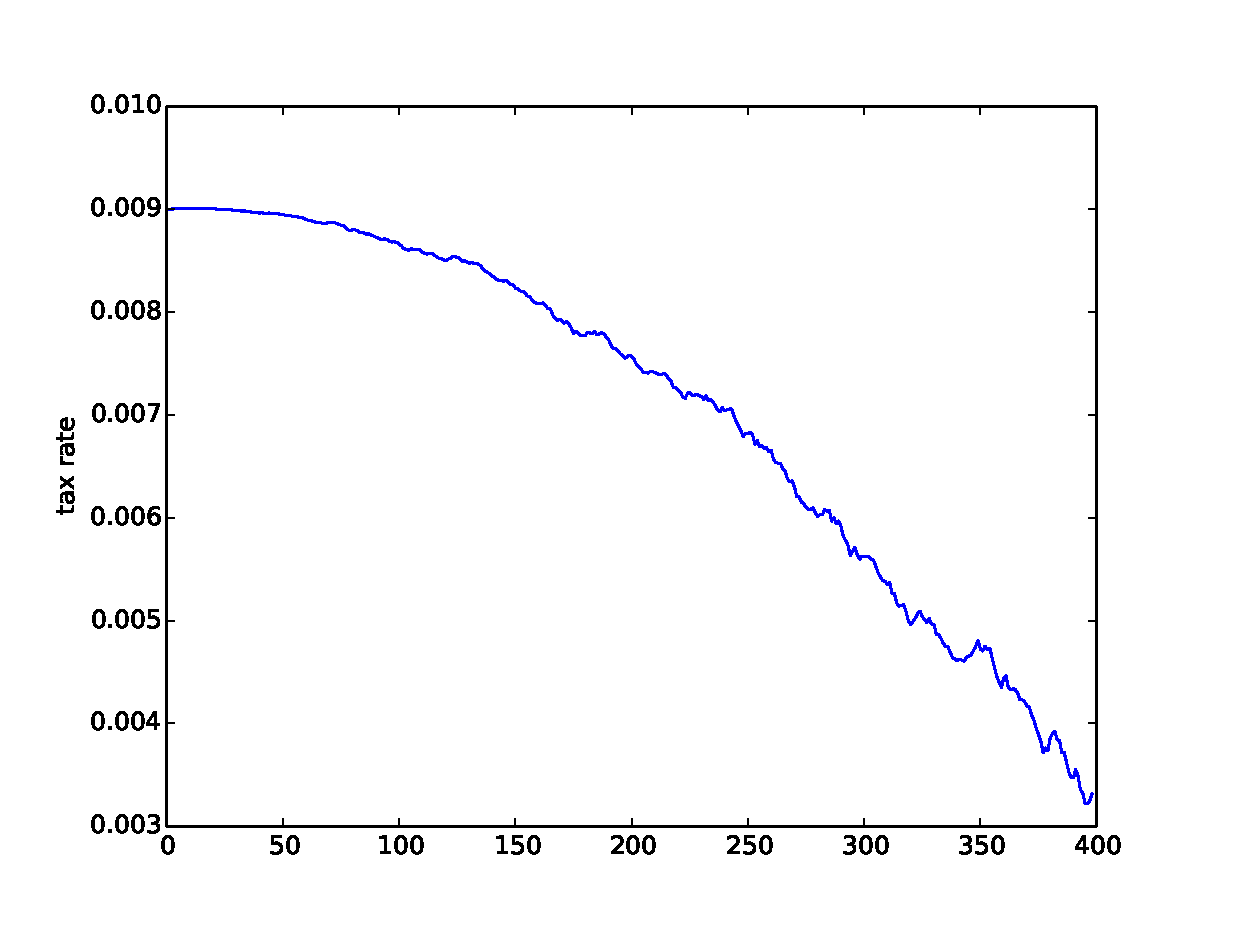
\includegraphics[width=\textwidth]{tax_iid.eps}
 \caption{Taxes in the iid economy.}
 \label{fig:taxes_iid}
 \end{figure}



  \begin{figure}[htp]
 \centering
 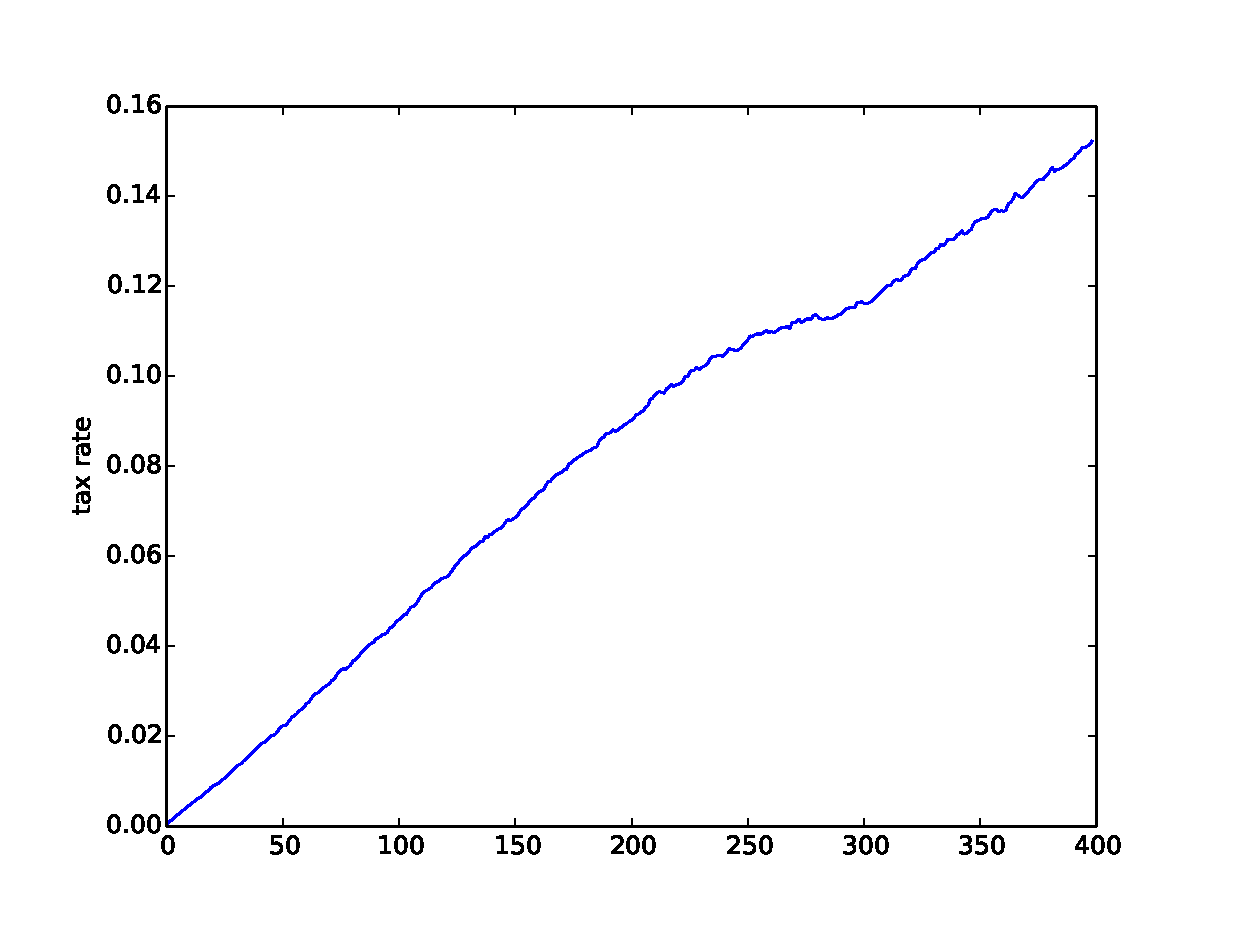
\includegraphics[width=\textwidth]{tax_pers.eps}
 \caption{Taxes in the unit root economy.}
 \label{fig:taxes_pers}
 \end{figure}




  \begin{figure}[htp]
 \centering
 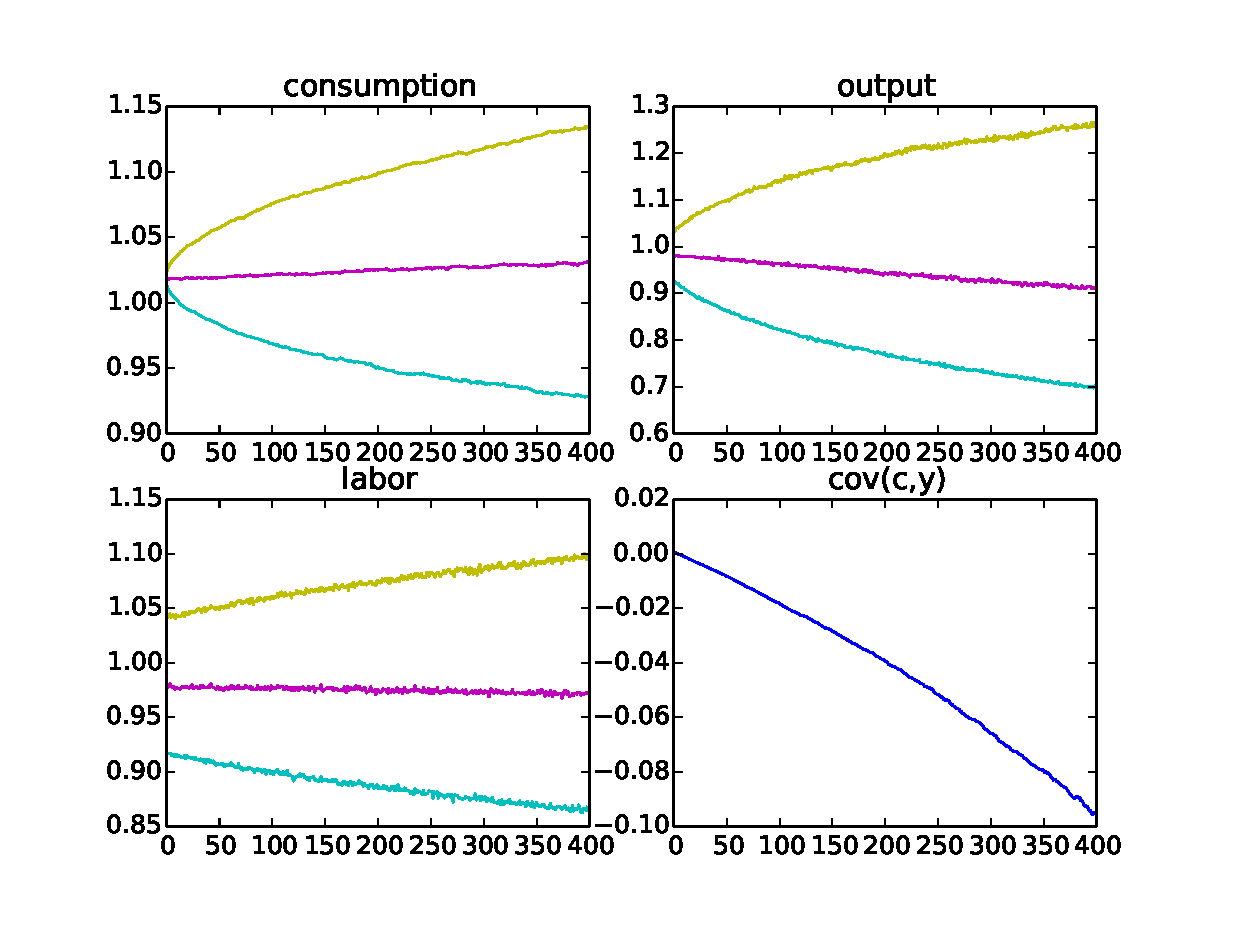
\includegraphics[width=\textwidth]{quant_iid.eps}
 \caption{Inequality in the iid economy. The figure plots the quantiles for consumption, pre-tax labor earnings, labor and the covariance between consumption and pre-tax labor earnings}
 \label{fig:quant_iid}
 \end{figure}



  \begin{figure}[htp]
 \centering
 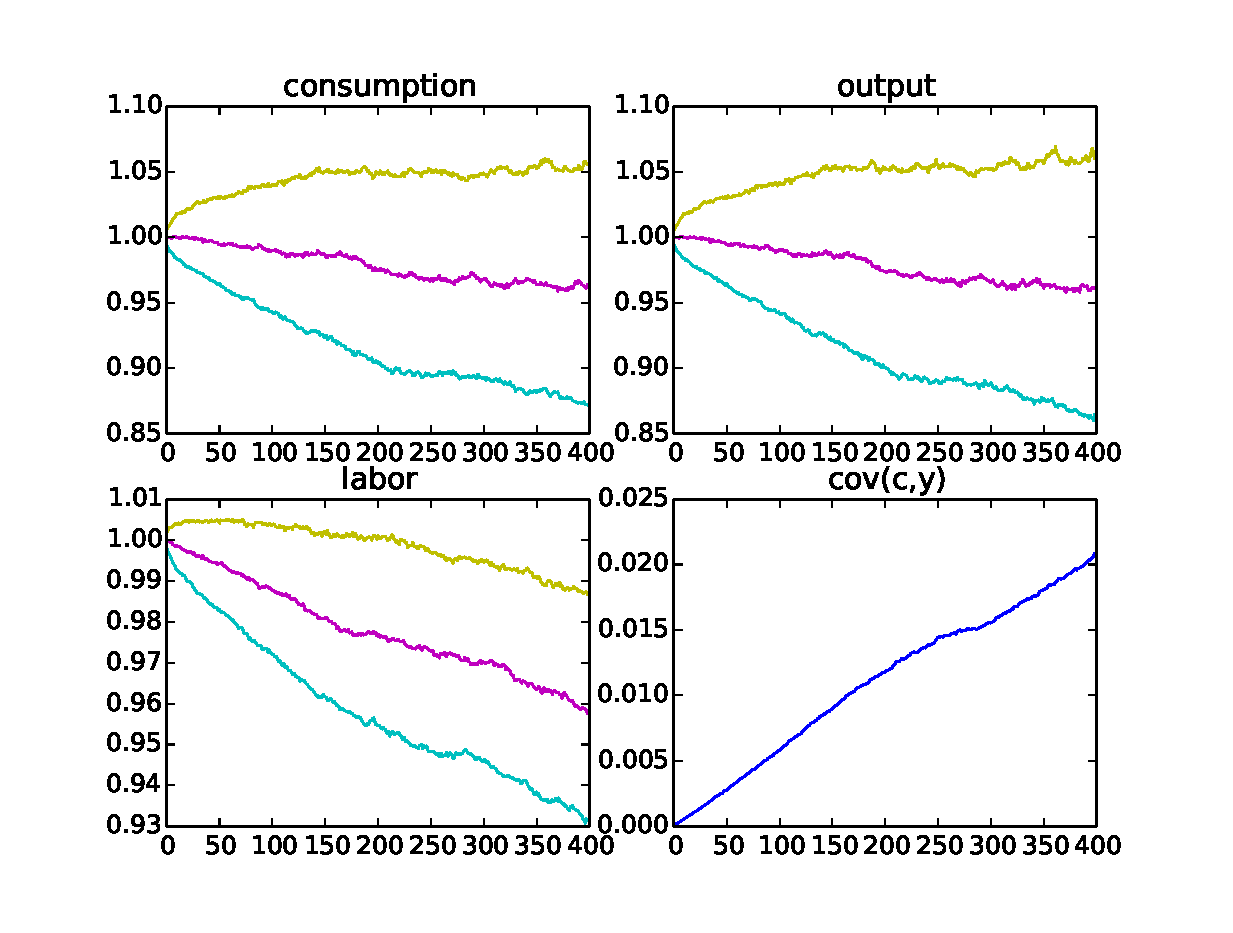
\includegraphics[width=\textwidth]{quant_pers.eps}
 \caption{Inequality in the unit root  economy. The figure plots the quantiles for consumption, pre-tax labor earnings, labor and the covariance between consumption and pre-tax labor earnings}
 \label{fig:quant_pers}
 \end{figure}




\section{Extentions}

  \begin{itemize}
  \item More realistic productivity process with common and idiosyncratic components. Something which generates earnings like in Fatih's paper.
  \item Adding capital 
  \item GHH preferences
  \end{itemize}

\section{Numerical Progress}
Currently we have an approximation to the time 1 problem for the following setup:
\begin{itemize}
	\item Government expenditures iid of the form
	\[
		g_t = g\exp(\eta_t)
	\]Though we are not restricted to government expenditure shocks, only to iid aggregate shocks for now.
	\item  Persistant idiosyncratic shocks
	\[
		e^i_t=(1-\nu)\bar{e}+\nu e^i_{t-1}+q\epsilon^i_t
	\]where $\nu \approx 1$.
\end{itemize}  This is done right now by taking the first order perturbation with respect to both $\nu$ and $\eta_t$.  Higher order approximations are doable but will take more time.  Figure \ref{fig:near_unit_quant} plots the quantiles of consumption labor and output for a calibration with no aggregate shocks and $\nu = 0.995$.  In addition Figure \ref{fig:near_unit_tax} plots a path of the labor tax rate with and without aggregate shocks.  The addition of aggregate shocks adds variability to the tax rate on top of the time path for the no-shock case.
\begin{figure}[htp]
\centering
	\includegraphics[width=0.8\textwidth]{near_unit_quant.eps}
	\caption{Inequality in the unit root  economy. The figure plots the quantiles for consumption, pre-tax labor earnings, labor and the covariance between consumption and pre-tax labor earnings\label{fig:near_unit_quant}}
\end{figure}
\begin{figure}[htp]
	\centering
	\includegraphics[width=0.49\textwidth]{near_unit_agg.eps}
	\includegraphics[width=0.49\textwidth]{near_unit_tax.eps}
	\caption{Time path of the tax rate with (left) and without (right) government expenditure shocks.\label{fig:near_unit_tax}}
\end{figure}
\newpage
\subsection{Calibration}
In terms of calibrating to the current US economy we propose the following:
\begin{enumerate}
	\item  Start with a joint distribution of assets and productivity or consumption and productivity.
	\item  Solve a complete markets problem with initial distribution of assets and productivities to match the distribution in the data.
	\item  This gives a distribution of multipliers and effective pareto weights we can use to simulate the incomplete markets economy. (we can also easily back out the time zero distribution of assets and productivities that would induce this choice so as to check if it is close to our initial distribution).
\end{enumerate}
\end{document}